\section{Introduction}
\label{sec:intro}

%Advances in 3D integrated circuits are enabling systems with DRAM dies stacked on top of logic chips~\cite{hmc, diram, jedec:high}. These systems with custom memory processing units (MPUs) are projected to enable significant improvements in bandwidth, latency, and energy. Consequently, researchers have begun proposing MPUs for many types of computation~\cite{ahn:scalable, gao:practical, pugsley:ndc, kim:neurocube, xi:beyond, power:implications, mirzadeh:sort} and coined the term {\it near-memory processing} for this computation paradigm. %Along with the inclusion of 3D memories in industry products~\cite{fujitsu:while, reinders:knights}, there is substantial evidence suggesting that future systems may consist of a pool of CPU and MPU-capable memory chips.

\djordje{I think the main points that need to come across are:
(1) Server workloads keep more and more data in memory --> server memory grows sharply in capacity
(2) Both compute and memory are scaling out due to the diminished scaling. Compute gets specialized resulting in a huge number of small execution units/accelerators, often placed close to memory ->  Maximum (and average) distance between logic and memory keeps increasing, while the minimum distance keeps decreasing. 
(3) The effectiveness of hardware translation gets worse as memory grows (TLB reach), and as the distance between memory and logic grows (page walk latency). More complex hardware needed to keep up with growing memory. 
(4) Small accelerators have *the same or worse* translation hardware requirements as large CPU cores --> a) the hardware overhead of translation is huge relative to a tiny accelerator, b) the overall translation hardware in the system scales linearly with the number of accelerators.  
(5) The overhead of TLB coherence gets worse as the system grows (I'd rather leave it for another section)

The net results are that translation HW requirements grow with the number of accelerators AND with memory capacity, with its effectiveness getting worse with both. 

We propose a scalable mechanism whose whose effectiveness does not depend on memory size or number of accelerators, and whose hardware requirements will not grow with the number of accelerators.
}

\javier{I don't like Djordje's story because all the points can be easily addressed by DVM. We need to explain the tradeoff between translation HW and SW flexility and a table comparing all the previous approaches. For example, DVM shows 4 variables: programmability, power/perf, flexibility, and safety. I think a simple way to drive the message home is that you want both (1) the programmability benefits of pointer-is-a-pointer
AND (2) flexible VM system (e.g., demand paging, COW), which is essentially what conventional address translation gives you. Then, we explain why it doesn't work for accelerators and we continue with SpryVM.}


Large-scale IT services are increasingly run in memory to accommodate tight query latency requirements. Online services rely on larger memory capacity to keep data closer to processing logic and faster processing to improve cost/performance and return on investment. In light of the slowdown in silicon efficiency and density scaling in recent years, designers are resorting to hardware accelerators for a wide spectrum of applications ranging from deep learning \cite{}, to analytics\cite{} and graph processing \cite{}. 

%\begin{figure*}[t]
%	\centering
%	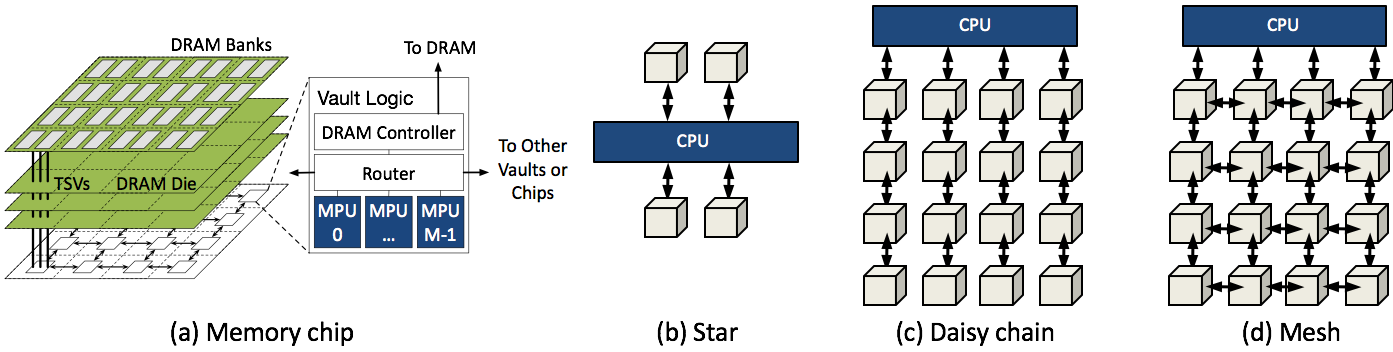
\includegraphics[width=0.85\textwidth]{figures/network.png}
%	\caption{Overview of a 3D memory architecture (a), and proposed and existing memory network topologies (b), (c), and (d).}
%	\label{fig:overview}
%\end{figure*}

%As with recent work on accelerators like GPUs~\cite{pichai:architectural, power:supporting}, a key research question is how virtual memory can be extended for MPUs. Enabling a unified virtual memory layer for CPUs and accelerators has many benefits: a simpler programming model, enabling "a pointer is a pointer everywhere" semantics~\cite{pichai:architectural, power:supporting, vesely:observation}, extending memory protection to accelerators, and obviating the need for manual inter-CPU-accelerator data marshalling. Vendors are already architecting unified virtual memory for GPUs (e.g., see AMD's Carrizo and Ryzen chips~\cite{wilcox:28nm}), with a view to generalizing it for all accelerators via the Heterogeneous System Architecture (HSA)~\cite{hsa}. Near-memory processing is following this integration path too~\cite{gao:practical, power:implications, xi:beyond}.

A salient feature of such accelerators is the need for a host CPU and OS to manage the execution resources among applications and application phases narrowing the scope of accelerator functionality to efficient and parallel in-memory computation. While many designers opt for accelerators to have direct physical access to memory, providing protection, isolation and the lack demand paging significantly complicates the software stack. Others have argued that the conventional virtual memory abstraction and a global address space programming model is best for software development enabling "a pointer is a pointer everywhere" semantics~\cite{pichai:architectural, power:supporting, vesely:observation}, extending memory protection to accelerators, and obviating the need for manual inter-CPU-accelerator data marshalling.


%Unfortunately, conventional virtual memory (VM) cannot simply be extended to MPUs without significant performance problems. The key culprit is virtual-to-physical address translation. Address translation performance is largely influenced by TLB capacity. As systems embrace ever-increasing memory sizes, it is difficult to design TLBs that provide adequate coverage of main memory. As a result, TLB misses are frequent, culminating in long-latency page table walks~\cite{pham:colt, pham:increasing, basu:efficient, karakostas:redundant, park:hybrid}. TLB overheads are known to be problematic for GPUs~\cite{pichai:architectural, power:supporting}, but we show that they are also detrimental to near-memory processing. Specifically, MPU TLB misses can be particularly long-latency because of the arbitrary distribution of page table entries across all the memory chips. Page table walks involve several chip-to-chip transfers of tens of nanoseconds per hop~\cite{huang:c3d, kanter:cavium, towles:unifying} for each level of the page table~\cite{gantz:hybrid}, incurring penalties of hundreds of nanoseconds. In other words, TLB overheads threaten to curtail the benefits of unified VM. 

Unfortunately, conventional virtual memory (VM) cannot simply be extended to accelerators. While general-purpose cores rely on deeper cache and TLB hierarchies and data reuse to bridge the gap between the core speed and memory capacity, accelerators primarily exploit parallel access with proximity to memory\cite{} forgoing reuse and deep hierarchies. The latter are also prohibitive in the required silicon resources relative to silicon-optimized accelerators. Moreover, accelerators are often designed to saturate the available memory bandwidth and are best placed near memory controllers, with physical memory partitioned among all accelerators to maximize parallelism\cite{}.


%The key culprit is virtual-to-physical address translation. Address translation performance is largely influenced by TLB capacity. As systems embrace ever-increasing memory sizes, it is difficult to design TLBs that provide adequate coverage of main memory. As a result, TLB misses are frequent, culminating in long-latency page table walks~\cite{pham:colt, pham:increasing, basu:efficient, karakostas:redundant, park:hybrid}. TLB overheads are known to be problematic for GPUs~\cite{pichai:architectural, power:supporting}, but we show that they are also detrimental to near-memory processing. Specifically, MPU TLB misses can be particularly long-latency because of the arbitrary distribution of page table entries across all the memory chips. Page table walks involve several chip-to-chip transfers of tens of nanoseconds per hop~\cite{huang:c3d, kanter:cavium, towles:unifying} for each level of the page table~\cite{gantz:hybrid}, incurring penalties of hundreds of nanoseconds. In other words, TLB overheads threaten to curtail the benefits of unified VM. Here we need to state that logic near memory can not afford deep TLB and cache hierarchies. Both the TLB reach and the page walk latency are key constraints.

Prior approaches to accommodate for accelerators either forgo VM and give direct physical access to memory for accelerators\cite{}, require major modifications to DRAM and memory controllers, or map physically contiguous regions of memory directly in VM or using segments\cite{}. These techniques fall short of providing the flexibility of a demand-paged VM and limit the utility of accelerators and/or introduce complex changes to the software stack.

%To address the problem, we observe that the main reason address translation impedes system performance is that it must complete before the subsequent data access. We take a back-to-basics approach and ask, is this serialization really necessary? In other words, is it possible to overlap memory translation with data fetch? By studying real-world server workloads, we identify that this decades-old serialized VM approach is an artifact of the early days of VM. In those days, memory was a scarce commodity and it was thereby necessary to enable a virtual page to map to any system page frame. This {\it fully associative} VM is flexible but requires memory translation to complete before data fetch.


In contrast, we propose {\it set-associative} VM, where a virtual page can map to one among a set of page frames. We dub this approach spryVM (Set-associative Page Regions of Your Virtual Memory). SpryVM restricts VM associativity so that a virtual address uniquely identifies the memory chip and partition that holds the data. This feature allows MPUs to access the memory as soon as the virtual address is known. Each memory partition integrates an MMU, which includes a TLB hierarchy and page table, that translates the virtual address and fetches the data---both the translation and data are always located in the MMU's local memory partition. SpryVM achieves low-overhead page walks as the page walk and data fetch operations overlap almost entirely. More specifically, our contributions are:

\noindent $\bullet$ A study of the VM associativity needs of modern server workloads. We are inspired by previous work on caches, which shows how associativity affects capacity, conflict, and compulsory misses \cite{hill:case}. 
We find that full VM associativity is often unnecessary, as most misses---page faults---are either compulsory or capacity, and are hence insensitive to associativity. Our study covers memory-resident and larger-than-memory working sets for single- and multi-programmed workloads.

%\item 
\noindent $\bullet$ A design space exploration for a hardware translation mechanism that leverages VM's modest associativity requirements. While such mechanisms do require OS changes, we show that these changes are readily-implementable as they can leverage existing and ongoing work on page coloring~\cite{mckusick:design}, multi-page table synchronization for heterogeneous memories~\cite{glisse:hmm}, and more. Moreover, we selectively apply set associativity to {\it regions} of the virtual address space that benefit from this approach. In so doing, we leave full-associativity for regions where it is better for performance, and retain cross-compatibility with existing systems.
%\item 

\noindent $\bullet$ SpryVM, a translation mechanism which restricts VM associativity so that a virtual address uniquely identifies a memory chip and partition, allowing MPUs to access the memory as soon as the virtual address is known. Each memory partition features an MMU, which includes a page table and TLB hierarchy to localize address translation and data fetch, thus minimizing the overhead. Each MMU's TLB hierarchy serves only its memory partition, makings its TLB performance robust across any memory chip and partition counts.

%\item 
\noindent $\bullet$ A comparison of spryVM with well-known translation mechanisms. SpryVM improves performance by up to $26\%$ and $15\%$ for in-memory and out-of-memory scenarios respectively, achieving almost-perfect zero-overhead address translation. 


\begin{comment}
Advances in 3D integrated circuits have enabled DRAM dies to be stacked on top of a logic chip~\cite{hmc, diram, jedec:high}. The projected benefits in bandwidth, latency, and energy have stimulated research and development of custom memory-side processing units (MPUs) on the logic chip for many different types of computation~\cite{ahn:scalable, gao:practical, pugsley:ndc, kim:neurocube, xi:beyond, power:implications, mirzadeh:sort}. Along with the inclusion of die-stacked memories in industry products~\cite{fujitsu:while, reinders:knights}, there is substantial evidence suggesting that future systems may consist of a pool of CPU and MPU-capable memory chips.

\begin{figure*}[t]
	\centering
	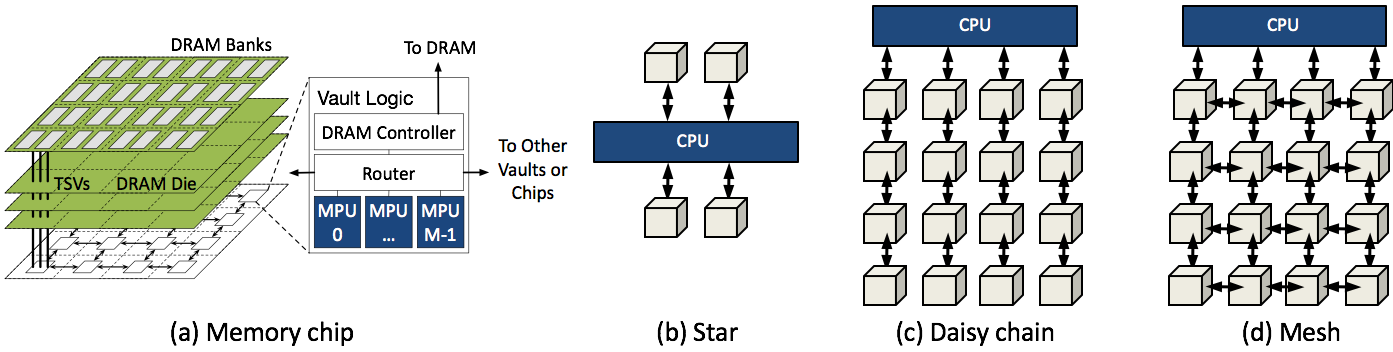
\includegraphics[width=0.85\textwidth]{figures/network.png}
	\caption{Overview of a 3D memory architecture (a), and proposed and existing memory network topologies (b), (c), and (d).}
	\label{fig:overview}
\end{figure*}

A key challenge in exploiting the full potential of these heterogeneous systems is the memory management between CPUs and MPUs. Industry initiatives such as the Heterogeneous System Architecture (HSA) Foundation are proposing to unify virtual memory (VM) between CPUs and any other processing unit in the system~\cite{hsa}. In this model, a pointer is equally valid on the CPU and MPU, simplifying data sharing and eliminating the need for explicit data copying and manual data consistency maintenance. In addition, VM enables efficient fine-grained memory accesses and transparent memory allocation and protection. Essentially, VM provides a familiar and powerful abstraction to programmers and operating systems alike. All these benefits have led HSA to adopt unified virtual memory into commercial GPUs, beginning with AMD's Carrizo chip~\cite{wilcox:28nm}. Given the benefits of HSA-style unified virtual memory and its early adoption and appearance in commercial products, we expect future computation units such as MPUs to also follow this integration path.

Unfortunately, the benefits of VM come at a significant performance overhead. Hardware support for address translation in commercial CPUs, which encompasses both per-core MMUs~\cite{intel:tlbs} and centralized IOMMUs for devices~\cite{intel:intel}, rely on TLB hierarchies that fall short of reaching the size of contemporary memories, resulting in frequent and long-latency page walks. Due to the arbitrary distribution of page table entries across all the memory chips, page walks involve several chip-to-chip transfers of tens of nanoseconds per hop~\cite{huang:c3d, kanter:cavium, towles:unifying} for each level of the page table~\cite{gantz:hybrid}, incurring in an unacceptable translation overhead of hundreds of nanoseconds. 

In this work, we observe that address translation stands on the critical path of accessing memory because a virtual page can map to any page frame---the mapping is fully associative. Hence, we perform an associativity study of VM (i.e., the number of locations that a virtual page can map to in the physical memory) across a variety of scenarios by classifying the page faults using the classic 3C model developed for caches~\cite{hill:aspects}. We conclude that capacity and compulsory misses---which are unaffected by associativity---dominate, while modest associativity is sufficient to eradicate conflict misses. More specifically, for working sets that are memory resident, compulsory misses dominate when the VM associativity equals the number of processes executing in the system. For working sets that exceed the memory size, capacity misses dominate and grow as a function of the working set size. In contrast, conflict misses become scarce once the associativity of virtual memory matches the number of processes in the system, and virtually disappear after the first few additional ways. Fundamentally, our associativity trends for VM match seminal work on set-associative caches~\cite{hill:aspects, cantin:cache}. 

We propose spryVM (Set-Associative Page Regions of your Virtual Memory), a VM system that restricts the associativity of VM so that a virtual address uniquely identifies a memory chip and partition. This feature allows MPUs to access the memory as soon as the virtual address is known. Each memory partition integrates an MMU, which includes a TLB hierarchy and page table, that translates the virtual address and fetches the data---both the translation and data are always located in the MMU's local memory partition. SpryVM achieves low-overhead page walks as the page walk and data fetch operations overlap almost entirely.

The primary contributions of this paper are:
%\begin{itemize}
%\item 

\noindent $\bullet$ A study of VM associativity using the 3C model. We show that full VM associativity is a largely unnecessary feature, as the majority of misses---page faults---are either compulsory or capacity, hence insensitive to associativity. Our study covers all scenarios: memory-resident and larger-than-memory working sets, single-process and multi-programmed. 

%\item 
\noindent $\bullet$ A design space exploration for a hardware translation mechanism that leverages VM's modest associativity requirements.
%\item 

\noindent $\bullet$ spryVM, a lightweight and high-performance translation mechanism which restricts VM associativity so that a virtual address uniquely identifies a memory chip and partition, allowing MPUs to access the memory as soon as the virtual address is known. Each memory partition features an MMU, which includes a page table and TLB hierarchy to localize address translation and data fetch, thus minimizing the overhead. 

%\item 
\noindent $\bullet$ An evaluation of spryVM against a set of state-of-the-art translation mechanisms. We show that our technique improves the performance of conventional address translation by up to $26\%$ and $15\%$ for in-memory and out-of-memory scenarios respectively, and almost eliminates the address translation overhead by performing within $1.2\%$ and $0.6\%$ of the ideal translation in each scenario respectively.
%\end{itemize}
\end{comment}

While we propose using set-associative VM to tackle the address translation challenges posed by MPUs, our key observations are general and likely useful for broader classes of multi-chip systems. Set-associativity is a general concept applicable to any system with  a significant memory access latency due to expensive chip-to-chip traffic. For instance, one could also envision the ideas of set-associativity and co-location of data and translation within the same memory partition/chip being applied to classic multi-socket NUMA machines~\cite{hp:hp, huawei:kunlun, ning:open}. We hope our study will inspire researchers to leverage set-associativity in other multi-chip systems.

%While we propose using set-associative VM to tackle the address translation challenges posed by MPUs, our key observations are general and likely useful for broader classes of multi-chip systems. Set-associativity is a general concept applicable to any system with  a significant latency gap between accesses to "local" and "remote" memories. In our context, "local" is analogous to intra-partition/chip, while "remote" corresponds to inter-partition/chip. For instance, one could also envision the ideas of set-associativity and co-location of data and translation within the same memory partition/chip being applied to classic multi-socket NUMA machines~\cite{hp:hp, huawei:kunlun, ning:open}. We hope our study will inspire researchers on leveraging set-associativity in other multi-chip systems.

%Overall, we believe that our study will shed light on how to leverage set-associativity in other multi-chip systems.

%We believe that our study on forward-looking systems with MPUs will ultimately shed light on how to apply and leverage set-associativity in other multi-chip systems.

% Please add the following required packages to your document preamble:
% \usepackage[table,xcdraw]{xcolor}
% If you use beamer only pass "xcolor=table" option, i.e. \documentclass[xcolor=table]{beamer}
\begin{table*}[]
\centering
\begin{tabular}{
>{\columncolor[HTML]{FFFFFF}}l |
>{\columncolor[HTML]{FFFFFF}}c |
>{\columncolor[HTML]{FFFFFF}}c |
>{\columncolor[HTML]{FFFFFF}}c |
>{\columncolor[HTML]{FFFFFF}}c |}
\cline{2-5}
\multicolumn{1}{c|}{\cellcolor[HTML]{FFFFFF}}                           & Programmability & Area and Power/Performance & Flexibility & Safety \\ \hline
\multicolumn{1}{|l|}{\cellcolor[HTML]{FFFFFF}Multi-page mappings}       & V               & X                          & V           & V      \\ \hline
\multicolumn{1}{|l|}{\cellcolor[HTML]{FFFFFF}Transparent Huge Pages}    & V               & X                          & V           & V      \\ \hline
\multicolumn{1}{|l|}{\cellcolor[HTML]{FFFFFF}libhugetlbfs}              & X               & X                          & V           & V      \\ \hline
\multicolumn{1}{|l|}{\cellcolor[HTML]{FFFFFF}Direct Segments}           & X               & V                          & X           & V      \\ \hline
\multicolumn{1}{|l|}{\cellcolor[HTML]{FFFFFF}Redundant Memory Mappings} & V               & X                          & X           & V      \\ \hline
\multicolumn{1}{|l|}{\cellcolor[HTML]{FFFFFF}Direct Mapped Mappings}    & V               & V                          & X           & V      \\ \hline
\multicolumn{1}{|l|}{\cellcolor[HTML]{FFFFFF}SpryVM}                    & V               & V                          & V           & V      \\ \hline
\end{tabular}
\end{table*}